% Preamble
% ---
\documentclass{article}

% Packages
% ---
\usepackage{amsmath} % Advanced math typesetting
\usepackage[utf8]{inputenc} % Unicode support (Umlauts etc.)
\usepackage{hyperref} % Add a link to your document
\usepackage{graphicx} % Add pictures to your document
\usepackage{listings} % Source code formatting and highlighting
\usepackage{framed} % Source code formatting and highlighting
\usepackage{appendix} % Source code formatting and highlighting
\usepackage{csquotes} % Pretty quotes
\usepackage{xcolor}
\usepackage{pagecolor}
\usepackage[letterpaper, portrait, margin=1.5in]{geometry}

\graphicspath{ {images/} }

\definecolor{limegreen}{HTML}{bbe963}


\title {XYO Cryptoeconomics and Tethering a Cryptocurrency to a Data Flow Index}

\author{
    Aaron Malone \thanks{Commonly known as "PizzaMind"}\\
    \and
    Arie Trouw\\
    \and    
    Bryce Paul\\
    \and
    Erik Saberski\\
    \and
    Nate Brune \thanks{Commonly known as "Machete"}\\
    \and
    Scott Scheper\\
}

\date{April 2019}

\begin{document}

\pagecolor{limegreen}

\maketitle

\begin{center}
\line(1,0){50}
\end{center}

\begin{abstract}
This document outlines the XYO Cryptoeconomics plan and sets forth an intriguing idea of tethering a cryptocurrency to \textit{data flow}. First, we provide supporting background knowledge of XYO's Token Economics. Then we lay forth the plan to grow XYO's network through handling the allocation of the GAMMA Token Pool. Finally, we lay forth an intriguing idea of tethering XYO to the amount of useful \textit{data flow} powering the network.
\end{abstract}

\section{Background}
The XYO Network is a cryptonetwork of IoT devices running an open protocol that provides valid and useful geospatial data to the world. The incentive mechanism powering the network is a cryptocurrency named "XYO".

We conducted the XYO Token Main Sale from March 20, 2018 - May 20, 2018. A total of 14,198,847,000 XYO was distributed through allocation and sale. The rest of the XYO Tokens were burned.

\subsection{The Cryptoeconomic Reserve}
We conducted the XYO Token Main Sale from March 20, 2018 - May 20, 2018. A total of 14,198,847,000 XYO was distributed through allocation and sale. The rest of the XYO Tokens were burned.

During the XYO Token Sale, a pool of XYO was created, called “The Cryptoeconomic Reserve”.

\begin{displayquote}\textit{``The goal of the Cryptoeconomic Reserve is to provide incentives to network participants in order to jump-start the foundation of the network.''} \cite{crypto-reserve}
\end{displayquote}

The Cryptoeconomic Reserve is for the following items:

\begin{enumerate}
  \item Incentivizing blockchain developers to create dApps that interact with XYO.
  \item Incentivizing Geominers (Operators of the four types of XYO Nodes: Sentinels, Bridges, Archivists and Diviners)
  \item Incentivizing XYO Token usefulness and network activity
  \item Facilitating decentralization amongst nodes
  \item Incentivizing artificial intelligence in nodes
\end{enumerate}


There is 2,871,068,696.85 XYO in the Cryptoeconomic Reserve (~2.8 Billion).

\subsection{GAMMA Token Pool}

5 billion XYO Tokens were allocated to a pool to be sold to the public. This ensured a decentralized XYO Token Pool (where the public owns and controls the majority of XYO). 

659,855,226.56 XYO was sold during the GAMMA Sale. The GAMMA Sale ended on November 30, 2018. The left-over amount of XYO is 4,340,144,773.44 in the GAMMA Token Pool.

\subsection{Founding HODL'er Registry (FHR)}

The FHR is comprised of those who \texttt{purchased} directly from the XYO Network core team from January 6, 2018 to November 30, 2018. See XIP-1.\cite{xip-1} The FHR List does not include any employees, partners, sponsors or individuals who received XYO for any reason. Only those who participated in the XYO Token Sales are included in the FHR.

One may view the FHR here: \textit{https://matrix.xyo.network/fhr}. Our XYO Founding HODL'ers form a special part of XYO's story and they're a huge reason for XYO's success!

\section{The Plan}

\subsection{XYO Token Distribution to FHR}

First, 340,144,773.44 XYO will be staked in the XYO Network with an un-staking period of 5 years. At the end of the period, the XYO can be withdrawn by the FHR Wallet Address. The XYO will be distributed on a pro rata basis, and is based on the amount of XYO you originally purchased.

\subsubsection{FHR Members}

If you are an XYO Founding HODL'er:

\begin{enumerate}
  \item The "H" in FHR stands for HODL.
  \item It is recommended that you hold the total amount of XYO you've bought in your FHR Wallet. 
  \item If you are unable to do this because you've since transferred it to a wallet in cold storage, that is OK \textit{as long as that cold storage wallet has at least the amount of XYO your purchased using the FHR Wallet}.
  \item We will be building a tool in the Matrix enabling you to white list wallet addresses that belong to you. In the meantime, we recommend you move your XYO back to your XYO FHR Wallet Address.
  \item Holding more XYO in your FHR Wallet Address than you purchased is also recommended. This will be factored into XYO reward multiples and Geodapp rewards. For example, if you purchased 100,000 XYO during the XYO Token Sale or in GAMMA, and you've since bought 50,000 more XYO), you may receive higher reward multiples if you hold 150,000 XYO in your FHR Wallet and stake that XYO. For this reason, we recommend you hold all of your XYO in your FHR Wallet (Reminder: Please keep your private keys secure).
  \item We intend to distribute XYO FHR NFT Tokens soon, which may make this process easier.
\end{enumerate}


\subsection{XYO Token Distribution to Cryptoeconomic Reserve}

With the XYO Mainnet launched and staking live, we will begin focusing on growing the XYO Network by using the Cryptoeconomic Reserve to acquire and train new customers (XYO Node Operators, aka "Geominers").

One of the ways we will deploy this is through selling XYO Cryptoeconomic Packages.

The remaining 4,000,000,000 in XYO from the GAMMA Token Pool will be allocated to the Cryptoeconomic Reserve. We will begin deploying this via the XYO Cryptoeconomic Packages covered next.

\subsection{XYO Cryptoeconomic Packages}

The XYO Cryptoeconomic Packages will contain the following items:

\begin{enumerate}
  \item XYO Tokens
  \item XYO Geominers (SentinelX's, XYO Bridges, Geomining Kits)
  \item 1 Geohacker Summit Ticket - Hosted Monthly in San Diego, CA (Teaching XYO Geomining and Node Operations)
  \item Dedicated VIP Concierge Phone Support and Training
  \item Cryptocurrency for gas and transfer fees when using the Matrix
  \item Plus more
\end{enumerate}

\subsubsection{Limited to One Package Per Customer}
In order to move towards network diversification (see the Cryptoeconomic Reserve section above), we are limiting each package to be purchased by customers on a one-time only basis.

\subsubsection{Limited to One Package Per Customer}
In order to move towards network diversification (see the Cryptoeconomic Reserve section above), we are limiting each package to be purchased by customers on a one-time only basis.

\subsubsection{XYO Sold via Cryptoeconomic Packages Includes Network Staking}

Every XYO Sold in Cryptoeconomic Packages use Network Staking.

This means, every XYO sold through the Cryptoeconomic Reserve has a staking period of 1-year (at minimum).

In the XYO Network, there are two types of staking. This is covered below. 

\subsection{XYO Staking: The Two Types}

\subsubsection{Network Staking}

The first type of staking is called \textit{Network Staking}. This comprises the act of staking your XYO for use in the XYO Network (between or amongst any nodes in the XYO Network). Once you execute a Network Stake, you lock your XYO in the ecosystem and can transfer the XYO between your own XYO nodes at any time. However, you cannot withdraw your XYO until the Network Stake Period has ended. 

This results in increased reward multiples whenever one pays for the bound witness data you generate. 

The minimum Network Stake Period is 1 year, although we recommend staking for much longer than that if you plan to hold XYO for the long-term.

Here is the Comparison of Values for Network Staking: (Green is 5 years)\\


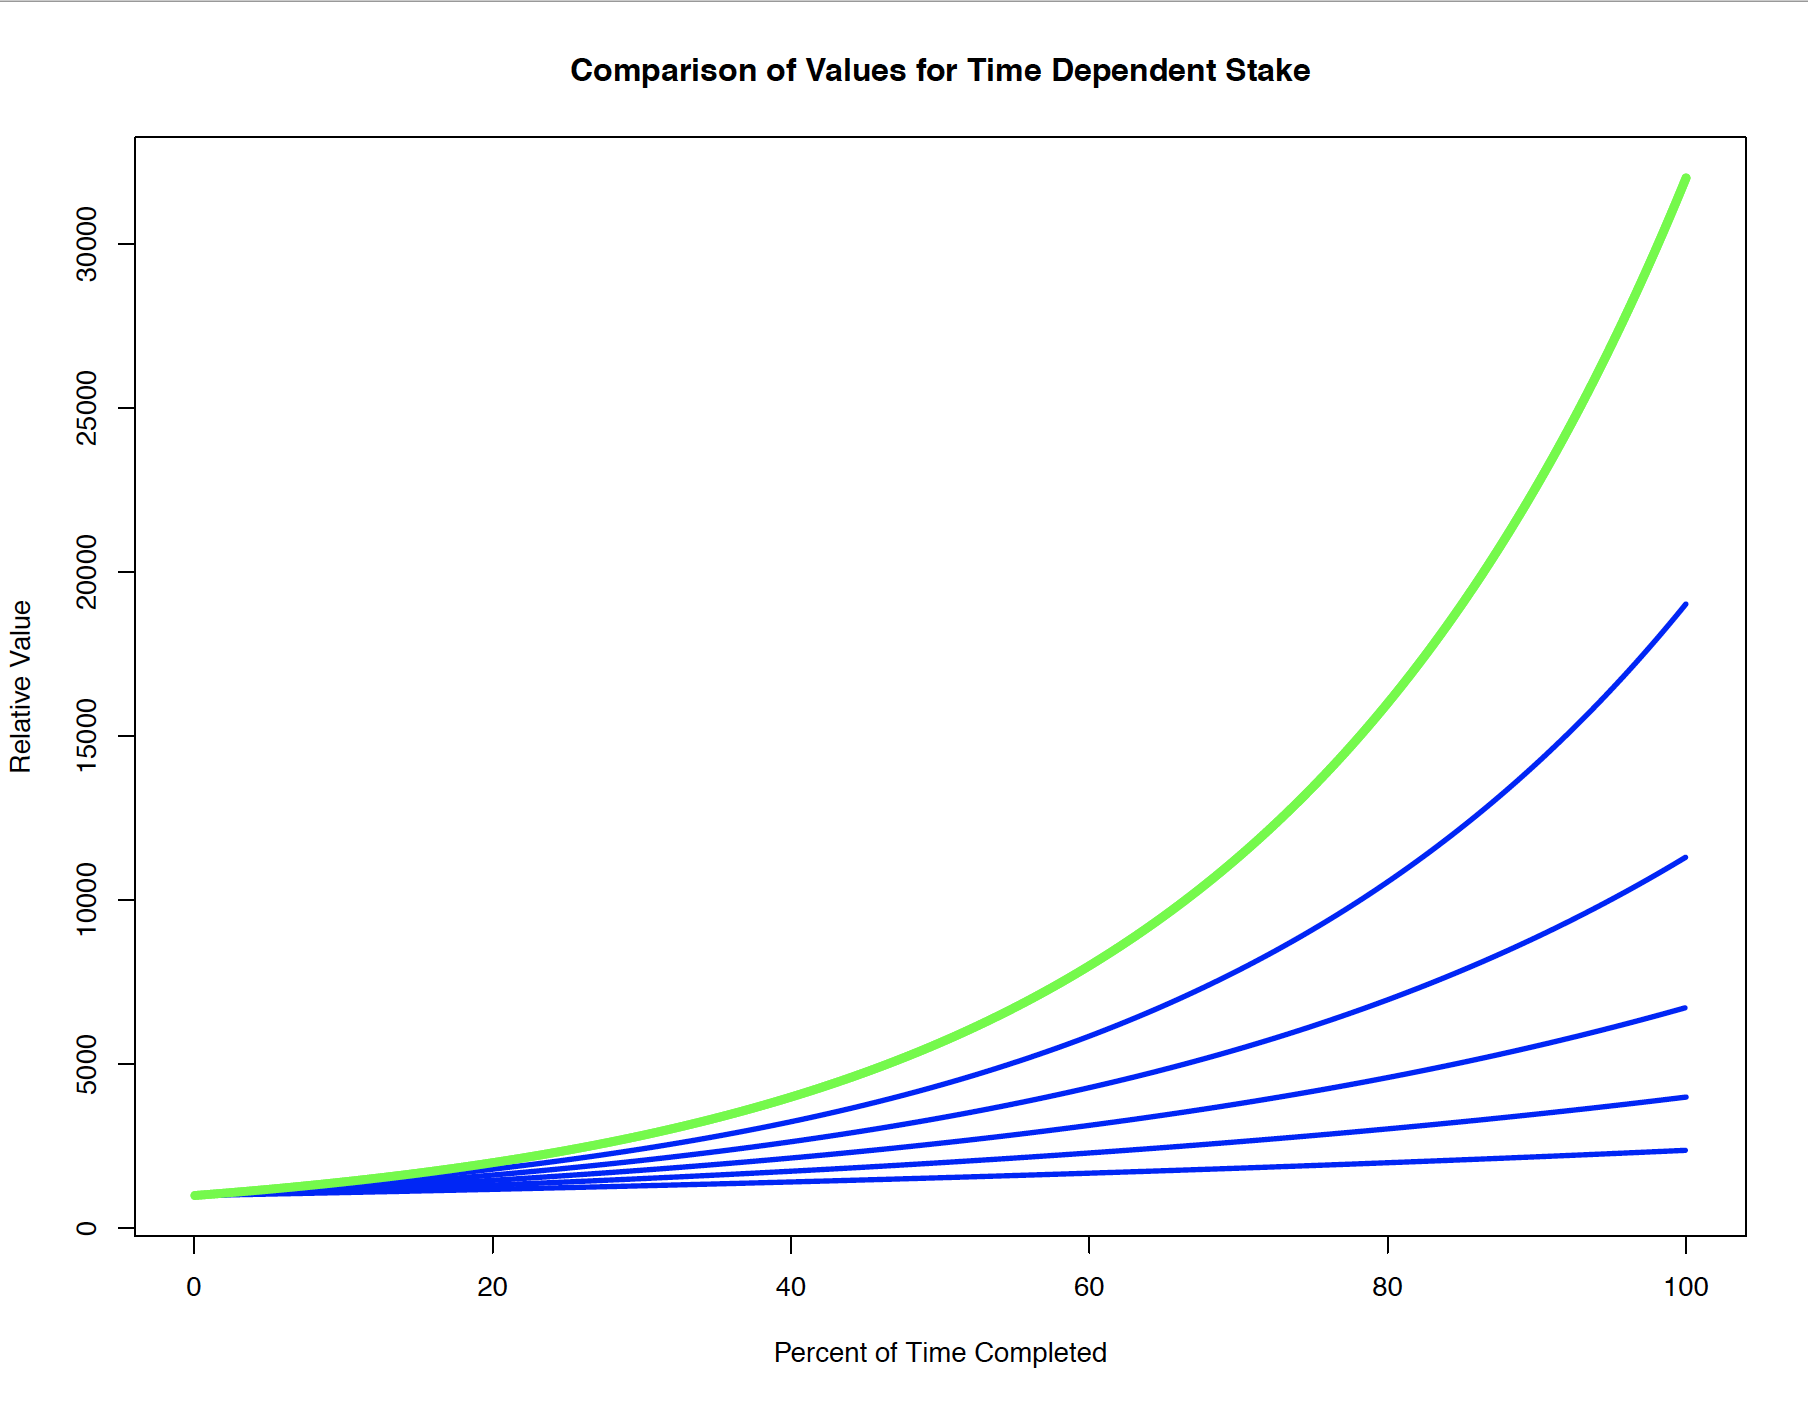
\includegraphics[width=\textwidth]{staking-time}

\subsubsection{Node Staking}

The second type of staking is called \textit{Node Staking}. This staking is conducted when you stake one of the four types of XYO Nodes (Sentinel, Bridge, Archivist, Diviner). 

Node-staking has a five-day unfreezing period. Meaning when you withdraw your XYO into your Ethereum ERC-20 Wallet, it takes five-days before it’s withdrawn from the network.

\subsubsection{Price of XYO}

Based on this, we will likely propose an XYO XIP to do the following:
After a certain period of time, if the XYO DFI model proves a solid indicator of XYO Network’s value, we will create a smart contract and that ties the value to a decentralized oracle that tracks the XYO DFI.

\begin{itemize}
  \item The starting point will be 10\% higher than the GAMMA Platform Sale Highest price (\$0.00942), which means we will be starting at \$0.01 per XYO.
  \item Pricing will be adjusted regularly according to the network growth, the XYO DFI (outlined below), and other factors.
  \item At a certain point in the future, if the XYO DFI model proves a solid indicator of XYO Network’s value, we will create a smart contract and that ties the value to a decentralized oracle that tracks the XYO DFI. During the Cryptoeconomic Reserve period, we will make constant adjustments to the DFI before finding the best fit for measuring the quality of data flow in the XYO Network.
\end{itemize}

\subsubsection{TODO's}

\begin{itemize}
  \item Erik Saberski: Staking Reward Mechanism
  \item Figure out DFI Formula
\end{itemize}

\begin{center}
\line(1,0){50}
\end{center}

\begin{thebibliography}{9}

\bibitem{crypto-reserve}
XYO Network
\\\texttt{https://xyo.network}.
March 2018.

\bibitem{xip-1}
XYO Improvement Protocol \#1
\textit{XYO Geohacker Forum}.
\\\texttt{https://geohackers.xyo.network/t/status-accepted-xip-1-founding-hodler-registry-fhr/927/104}.
March 2018.

\end{thebibliography}

%*******************************
%**** End Glossary Section *****
%*******************************

\end{document}
